\documentclass[12pt]{article}

\usepackage{hcmus-report-template}

% Disable indentation on new paragraphs
\setlength{\parindent}{0pt}

% Line spacing 1.5
\renewcommand{\baselinestretch}{1.5}

% Optional: graphic path
% \graphicspath{PATH_TO_GRAPHIC_FOLDER}

% To use Times font family, uncomment this row
% \usepackage{mathptmx}

% To use roman section / subsection, uncomment these rows
% \renewcommand{\thesection}{\Roman{section}}
% \renewcommand{\thesubsection}{\thesection.\Roman{subsection}}

% Define course name, report name and report title.
\newcommand{\coursename}{CS163 - Data Structures}
\newcommand{\reportname}{Sorting Algorithms}
\newcommand{\reporttitle}{Seminar Report}

% Define student name and teacher name.
\newcommand{\studentname}{Thuan, Le Minh - 24125105\\ Phu, Nguyen Minh - 24125103 \\ Lac, Quach Thien - 24125092\\ Quan, Pham Nguyen Minh - 24125041}
\newcommand{\teachername}{MSc. Thanh, Ho Tuan\\ MSc. Loc, Truong Phuoc}

% Header
\lhead{\reporttitle}
\rhead{
VNU-HCM University of Science\\
\coursename
}

% Footer
% \newcommand{\leftfooter}{\LaTeX\ by }
% \lfoot{\leftfooter}

% ============ DOCUMENT ============
\begin{document}

\pagenumbering{roman}
\begin{titlepage}
\newcommand{\HRule}{\rule{\linewidth}{0.5mm}}
\centering

\textsc{\LARGE Viet Nam National University}\\[0.5cm]
\textsc{\LARGE Ho Chi Minh City}\\[0.5cm]
\textsc{\Large University of Science}\\[0.5cm]
\textsc{\large \textbf{Faculty of Information Technology}}\\[0.5cm]

\HRule \\[0.4cm]
{ 
\huge{\bfseries{\reporttitle}}\\[0.5cm]
\large{\bfseries{Subject: \reportname}}
}\\[0.4cm]
\HRule \\[0.5cm]

\textbf{\large Course: \coursename}\\[0.5cm]

\begin{minipage}[t]{0.5\textwidth} % Adjusted width
\begin{flushleft} \large
\emph{Group 05 - 24A02:}\\
\studentname
\end{flushleft}
\end{minipage}
~
\begin{minipage}[t]{0.4\textwidth} % Adjusted width
\begin{flushright} \large
\emph{Supervisors:} \\
\teachername
\end{flushright}
\end{minipage}\\[1cm]

{\large \today}\\[1cm]

\vfill
\end{titlepage}


\tableofcontents
\pagebreak
% \listoftables
% \pagebreak
\listoffigures
\pagebreak

\pagenumbering{arabic}
\setcounter{page}{1}

% \section{Section}

\subsection{Một số lưu ý}

\subsubsection{Cài đặt offline}
Template này yêu cầu cài đặt một số gói (package) nâng cao cho TexStudio:
\begin{itemize}
\item Để gõ thuật toán: \texttt{algorithm} và \texttt{algpseudocode}
\item Để nhúng (chèn) code: \texttt{listings}
\end{itemize}
Các gói này được cài đặt thông qua lệnh
\begin{lstlisting}[language=sh]
sudo apt-get install texlive-full
\end{lstlisting}
Tuy nhiên kích thước gói đâu đó vào khoảng 5GB (!). Vì vậy tốt nhất nên xài Overleaf.

\subsubsection{Sử dụng font khác}
Tham khảo font typefaces tại \href{https://www.overleaf.com/learn/latex/Font_typefaces}{link này}.

\subsubsection{Đánh số chỉ mục bằng chữ số La Mã}
Mở file \texttt{main.tex} và bỏ comment dòng 
\begin{lstlisting}[language=tex]
% \renewcommand{\thesection}{\Roman{section}}
% \renewcommand{\thesubsection}{\thesection.\Roman{subsection}}  
\end{lstlisting}

\subsection{Ví dụ}
Ngày xửa ngày xưa, ở vương quốc VNUHCM - US, có một chàng hoàng tử ngồi cắm đầu viết doc\footnote{Đây là footnote, chú thích lại những gì cần chú ý.}.\\
Mặc định muốn xuống dòng chỉ cần dùng $\backslash\backslash$  (2 lần dấu xẹt huyền).\\
Nếu bạn muốn thụt đầu dòng khi bắt đầu paragraph mới, vào \texttt{main.tex} và disble dòng
\begin{lstlisting}[language=tex]
\setlength{\parindent}{0pt}
\end{lstlisting}

\subsection{First subsection}
\subsubsection{First sub-subsection}
Subsection để ví dụ thôi. Thêm vài ví dụ:
\begin{itemize}
    \item Dùng itemize
    \item Vẫn là itemize
\end{itemize}
Sau đó xài enumerate:
\begin{enumerate}
    \item Dùng enumerate
    \item Vẫn là enumerate
\end{enumerate}
Nhỏ hơn subsubsection thì xài \texttt{paragraph}:

\paragraph{Đây là ví dụ cho paragraph}
Lưu ý là paragraph không nằm trong Mục lục.

\subsection{Chia nhỏ nội dung}
Bạn có thể chia nhỏ nội dung của báo cáo thành các file \texttt{.tex} và dùng lệnh \texttt{input} để chèn vào báo cáo chính. Ví dụ có trong file \texttt{main.tex}.
% \section{Hình ảnh}
Hình ảnh được thể hiện như hình~\ref{fig:my_label}, lưu ý flag \texttt{[H]} để disable floating (hình được hiển thị đúng vị trí, không trôi lên đầu trang).
\begin{figure}%[H]
\centering

\includegraphics[scale=.4]{img/hcmus-logo.png}
\caption{Hình ví dụ (logo HCMUS - updated 30/11/2022)}
\label{fig:my_label}
\end{figure}

Hình~\ref{fig:my_label_with_H} cũng là hình ví dụ nhưng có tag \texttt{[H]}. Lưu ý là có tag \texttt{[H]} thì code ở đâu hình sẽ nằm ở đó, không quan trọng nội dung ít hay nhiều (trang giấy sẽ thừa 1 khúc như bạn thấy). Để hiểu hơn về positioning trong LaTeX, xin tham khảo \href{https://www.overleaf.com/learn/latex/Positioning_images_and_tables}{bài này}.

\begin{figure}[H]
\centering

\includegraphics[scale=.4]{img/hcmus-logo.png}
\caption{Hình ví dụ (logo HCMUS - updated 30/11/2022)}
\label{fig:my_label_with_H}
\end{figure}
% \section{Bảng biểu}
Bảng biểu được thể hiện như bảng~\ref{tab:my_label}, lưu ý flag \texttt{[H]} để disable floating (bảng được hiển thị đúng vị trí, không trôi lên đầu trang). Bảng~\ref{tab:my_label} là một trường hợp không sử dụng tag \texttt{[H]} và bảng bị trôi tít lên đầu trang:
\begin{table}%[H]
\centering
\begin{tabular}{|l|l|}
\hline
\textbf{Tên con vật} & \textbf{Số chân} \\ \hline
Gà & 2 \\ \hline
Chó & 4 \\ \hline
Trần Hoàng Tử & 2 \\ \hline
\end{tabular}
\caption{Số chân của một số con vật, không có tag \texttt{[H]}}
\label{tab:my_label}
\end{table}

Bảng~\ref{tab:my_label_with_H_tag} thể hiện bảng biểu với tag \texttt{[H]}\footnote{Tương tự cách sử dụng tag \texttt{[H]} với hình}. Để không phải mất thời gian tuổi trẻ ngồi chỉnh table, xài \href{https://www.tablesgenerator.com}{https://www.tablesgenerator.com}.

\begin{table}[H]
\centering
\begin{tabular}{|l|l|}
\hline
\textbf{Tên con vật} & \textbf{Số chân} \\ \hline
Gà & 2 \\ \hline
Chó & 4 \\ \hline
Trần Hoàng Tử & 2 \\ \hline
\end{tabular}
\caption{Số chân của một số con vật, có tag \texttt{[H]}}
\label{tab:my_label_with_H_tag}
\end{table}.
% \section{Công thức toán}
Công thức toán gõ chung 1 dòng thì dùng 2 lần dấu dollar: $f(x) = x^2 + 2x + 1$. Với công thức nằm riêng 1 dòng thì gõ 2 cặp dấu dollar:
$$
ReLU(x) = \max(0, x)
$$
Siêu việt hơn, gõ hệ phương trình thì nên dùng tag \texttt{equation}
\begin{equation*}
\begin{aligned}
a_1x_1 + a_2x_2 + .. + a_nx_n &= u \\
b_1x_1 + b_2x_2 + .. + b_nx_n &= v \\
c_1x_1 + c_2x_2 + .. + c_nx_n &= w \\
\end{aligned}
\end{equation*}
Tham khảo cách gõ equation trên \href{https://www.overleaf.com/learn/latex/Mathematical_expressions}{Overleaf} nhé!
\section{Heap Sort}

\subsection{Introduction}
\textbf{History:} Heap Sort was first introduced by J.W.J. Williams in 1964. This innovation aimed to exploit the heap data structure to improve sorting performance.

\begin{figure}[H]
\centering
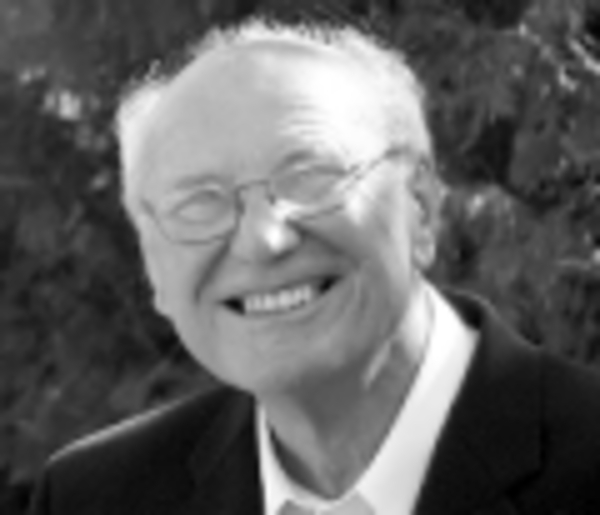
\includegraphics[scale=.3]{img/jwjWilliams.jpg}
\caption{J. W. J. Williams (1930-2012)}
\label{fig:jwj_williams}
\end{figure}

\textbf{Definition:} Heap Sort is a comparison-based, in-place sorting algorithm that leverages the properties of a heap data structure—specifically, a max heap when sorting in ascending order. Its basic premise is:
\begin{enumerate}
    \item \textbf{Max Heap Property:} In a max heap, every parent node is greater than or equal to its children. This guarantees that the largest element is always at the root.
    \item \textbf{In-Place Sorting:} Heap Sort rearranges the data within the input array, meaning it does not require significant additional memory.
    \item \textbf{Time Complexity:} It consistently operates in $O(n \log n)$ time in the worst case, making it reliable and predictable.
\end{enumerate}

\subsection{Algorithm and Implementation}

\textbf{Step 1: Build the Max Heap}
\begin{itemize}
    \item \textbf{Determine the Starting Point:}
    \begin{itemize}
        \item The array is treated as a complete binary tree.
        \item The last non-leaf node resides at index $\lfloor n/2 \rfloor - 1$, where $n$ is the total number of elements.
    \end{itemize}
    \item \textbf{Call heapify() on Each Non-Leaf Node:}
    \begin{itemize}
        \item Starting from the last non-leaf node and moving upward to the root, apply the heapify() procedure to enforce the max heap property.
        \item The heapify() procedure ensures that for a node at index $i$, the value at $i$ is greater than or equal to its children.
    \end{itemize}
\end{itemize}

\begin{algorithm}
    \caption{Heapify}
    \begin{algorithmic}[1]
        \State \textbf{Input:} Array $A$, index $i$, size $n$
        \State \textbf{Output:} Array $A$ with max heap property enforced at index $i$
        \Function{Heapify}{$A$, $i$, $n$}
        \State $largest \gets i$
        \State $left \gets 2i + 1$
        \State $right \gets 2i + 2$
        \If{$left < n$ \textbf{and} $A[left] > A[largest]$}
        \State $largest \gets left$
        \EndIf
        \If{$right < n$ \textbf{and} $A[right] > A[largest]$}
        \State $largest \gets right$
        \EndIf
        \If{$largest \neq i$}
        \State \Call{Swap}{$A[i]$, $A[largest]$}
        \State \Call{Heapify}{$A$, $largest$, $n$}
        \EndIf
        \EndFunction
    \end{algorithmic}
\end{algorithm}

\begin{algorithm}
    \caption{BuildMaxHeap}
    \begin{algorithmic}[1]
        \State \textbf{Input:} Array $A$
        \State \textbf{Output:} Array $A$ transformed into a max heap
        \Function{BuildMaxHeap}{$A$}
        \State $n \gets |A|$
        \For{$i \gets \lfloor n/2 \rfloor - 1$ \textbf{downto} 0}
        \State \Call{Heapify}{$A$, $i$, $n$}
        \EndFor
        \EndFunction
    \end{algorithmic}
\end{algorithm}

\textbf{Step 2: Sort the Array (Extract Elements from Heap)}
\begin{itemize}
    \item \textbf{Swap the Root with the Last Element:}
    \begin{itemize}
        \item The root of the max heap (index 0) holds the maximum value. Swap it with the last element in the heap (at index $n-1$).
    \end{itemize}
    \item \textbf{Reduce Heap Size:}
    \begin{itemize}
        \item After the swap, consider the last element as sorted. Reduce the effective heap size by one so that it is excluded from further heap operations.
    \end{itemize}
    \item \textbf{Re-heapify the Root:}
    \begin{itemize}
        \item Call the heapify() procedure on the root (index 0) to restore the max heap property over the reduced heap.
    \end{itemize}
    \item \textbf{Repeat Extraction:}
    \begin{itemize}
        \item Continue this process, swapping the root with the last unsorted element and re-heapifying until the entire array is sorted.
    \end{itemize}
\end{itemize}

\begin{algorithm}
    \caption{HeapSort}
    \begin{algorithmic}[1]
        \State \textbf{Input:} Array $A$
        \State \textbf{Output:} Sorted array $A$
        \Function{HeapSort}{$A$}
        \State \Call{BuildMaxHeap}{$A$}
        \For{$i \gets |A| - 1$ \textbf{downto} 1}
        \State \Call{Swap}{$A[0]$, $A[i]$}
        \State \Call{Heapify}{$A$, 0, $i$}
        \EndFor
        \EndFunction
    \end{algorithmic}
\end{algorithm}

\begin{minipage}{\linewidth}
    Below is the implementation in C++:

    \lstinputlisting[language=C++, caption=Heap Sort in C++, style=mystyle]{code/heapSort.cpp}    
\end{minipage}

\subsection{Evaluation}

\subsubsection{Building the Heap}
\textbf{Operation:} Constructing a Heap (Max-Heap) from the input array. \\
\textbf{Complexity:} $O(n)$ \\
\textbf{Explanation:} While a single “heapify” operation takes $O(\log n)$, the total time to build the heap is $O(n)$ due to optimization when handling elements at lower levels of the heap.

\subsubsection{Extracting Elements from the Heap}
\textbf{Operation:} Extract the root element (maximum) and rearrange the heap. \\
\textbf{Complexity:} $O(n \log n)$ \\
\textbf{Explanation:} There are $n$ extractions, and each extraction is followed by a "heapify" operation that takes $O(\log n)$.

\subsubsection{In-Place Sorting}
\textbf{Operation:} Swap the extracted root element with the last unsorted element. \\
\textbf{Complexity:} $O(n \log n)$ \\
\textbf{Explanation:} Swapping is combined with extraction and re-heapification, contributing to the overall complexity.

\subsubsection{Space Complexity}
\textbf{Space Used:} $O(1)$ \\
\textbf{Explanation:} Heap Sort is an in-place sorting algorithm, so it does not require additional space beyond the input array.

\subsection{Application}

Heap sort is a strong algorithm. It has several practical applications due to its efficiency and predictable performance:
\begin{enumerate}
    \item \textbf{Sorting Large Datasets:} Heap sort is particularly useful for sorting large datasets where memory usage is a concern. \textit{Example:} Sorting a large database of employee records by salary.
    \item \textbf{Priority Queue Implementation:} Heap sort is the foundation for implementing priority queues. Priority queues are used in scheduling algorithms, such as in operating systems or task management systems. \textit{Example:} Scheduling tasks in a CPU based on their priority levels.
    \item \textbf{External Sorting:} Heap sort is used in external sorting algorithms where data is too large to fit into memory. It helps in merging sorted chunks of data efficiently. \textit{Example:} Sorting large files stored on disk.
    \item \textbf{Real-Time Systems:} Heap sort is used in real-time systems where predictable performance is critical. \textit{Example:} Sorting sensor data in real-time for autonomous vehicles.
    \item \textbf{Selection Algorithms:} Heap sort is used in selection algorithms to find the $k$th smallest or largest element in a list. \textit{Example:} Finding the median of a dataset efficiently.
    \item \textbf{Game Development:} Heap sort is used in game development for managing and sorting game objects based on priority or distance. \textit{Example:} Rendering objects in a game based on their distance from the camera.
    \item \textbf{Event-Driven Simulations:} Heap sort is used in simulations where events need to be processed in a specific order. \textit{Example:} Simulating the behavior of a queue in a bank or a call center.
    \item \textbf{Operating Systems:} Heap sort is used in operating systems for memory management and process scheduling. \textit{Example:} Managing memory allocation for processes in a multi-tasking environment.
\end{enumerate}

\subsection{Problems}

\subsubsection{Kth Largest Element in an Array}
\href{https://leetcode.com/problems/kth-largest-element-in-an-array/}{LeetCode}

\textbf{Description:} Given an unsorted array, determine the $k$th largest element.

\textbf{Detailed Instructions:}
\begin{enumerate}
    \item Create a min-heap (priority queue) and insert the first $k$ elements of the array into it.
    \item For every remaining element in the array, compare it with the heap’s root. If it’s larger, remove the root and insert the new element, maintaining the heap property.
    \item Once all elements are processed, the root of the heap is the $k$th largest element. Use this technique to optimize your time complexity to $O(n \log k)$.
\end{enumerate}

\subsubsection{Find Median from Data Stream}
\href{https://leetcode.com/problems/find-median-from-data-stream/}{LeetCode}

\textbf{Description:} Continuously find the median of a stream of numbers.

\textbf{Detailed Instructions:}
\begin{enumerate}
    \item Use two heaps: a max-heap for the lower half of the numbers and a min-heap for the upper half.
    \item When a new number arrives, decide which heap to insert it into, then rebalance the heaps if their sizes differ by more than one.
    \item For median retrieval, if heaps are equal in size, average the roots; otherwise, return the root of the larger heap. This dual-heap method ensures that the median is found efficiently after each insertion.
\end{enumerate}

\subsubsection{Merge k Sorted Lists}
\href{https://leetcode.com/problems/merge-k-sorted-lists/}{LeetCode}

\textbf{Description:} Merge multiple sorted linked lists into one sorted linked list.

\textbf{Detailed Instructions:}
\begin{enumerate}
    \item Initialize a min-heap and insert the head (first node) of each of the $k$ lists into it.
    \item Repeatedly extract the smallest node from the heap and append it to the merged list. If the extracted node has a next node, insert that node into the heap.
    \item Continue until the heap is empty. This process ensures that at each step, you’re adding the smallest current node, maintaining overall sorted order.
\end{enumerate}

\subsubsection{Sliding Window Median}
\href{https://leetcode.com/problems/sliding-window-median/}{LeetCode}

\textbf{Description:} Given an array and a window size $k$, compute the median of every sliding window.

\textbf{Detailed Instructions:}
\begin{enumerate}
    \item Use two heaps (max-heap and min-heap) to represent the current window’s lower and upper halves.
    \item As the window slides, add the new element and remove the element that’s moving out of the window. Rebalance the heaps to maintain the required size properties.
    \item After every slide, compute the median based on the roots of the two heaps. This ensures an efficient update and retrieval of the median as the window moves.
\end{enumerate}
\section{Counting Sort}

\subsection{Introduction}
\textbf{History:}
Counting Sort was developed by Harold H. Seward in the early 1950s, often cited around 1954. It is recognized for its ability to sort integers in linear time under the right conditions.

\begin{figure}[H]
\centering
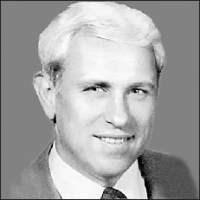
\includegraphics[scale=1]{img/haroldHSeward.jpg}
\caption{Harold H. Seward (1930-2012)}
\label{fig:harold_h_seward}
\end{figure}

\textbf{Definition:}
Counting Sort is a non-comparison-based sorting algorithm that sorts elements by counting the number of occurrences of each unique value in the input array. It then uses these counts to determine the positions of each element in the final, sorted array.

\begin{itemize}
    \item The algorithm operates in linear time.
    \item Time complexity: \(O(n + k)\), where \(n\) is the number of elements and \(k\) is the range of the input values.
\end{itemize}

\subsection{Algorithm and Implementation}
\begin{enumerate}
    \item \textbf{Determine the Range of the Data:} Sometimes min is assumed to be 0 to simplify the process.
    \item \textbf{Initialize the Count Array:} Create a count array of size \((\text{max} - \text{min} + 1)\) and initialize all elements to 0.
    \item \textbf{Count the Occurrences:} Iterate over the input array and for each element, increment the corresponding index in the count array. For an element \(x\), increment \(\text{count}[x - \text{min}]\).
    \item \textbf{Transform the Count Array into a Cumulative Count Array:} Modify the count array such that each element at index \(i\) contains the sum of previous counts. This cumulative count tells you the final position of each element in the output array.
    \item \textbf{Build the Output Array:}
    \begin{itemize}
        \item Traverse the input array once more, usually in reverse order to ensure stability (maintaining the original order of equal elements).
        \item Place each element \(x\) into its correct position in the output array by using the cumulative count, then decrement the count value for \(x\).
    \end{itemize}
\end{enumerate}

\begin{algorithm}
\caption{Counting Sort}
\begin{algorithmic}[1]
\State \textbf{Input:} Array $A$ of size $n$
\State \textbf{Output:} Sorted array $B$
\State \textbf{Determine the Range of the Data}
\State $min \gets \min(A)$
\State $max \gets \max(A)$
\State \textbf{Initialize the Count Array}
\State $count \gets \text{array of size } (max - min + 1) \text{ initialized to 0}$
\State \textbf{Count the Occurrences}
\For{each element $x$ in $A$}
    \State $count[x - min] \gets count[x - min] + 1$
\EndFor
\State \textbf{Transform the Count Array into a Cumulative Count Array}
\For{$i \gets 1$ to $length(count) - 1$}
    \State $count[i] \gets count[i] + count[i - 1]$
\EndFor
\State \textbf{Build the Output Array}
\State $B \gets \text{array of size } n$
\For{each element $x$ in $A$ \textbf{in reverse order}}
    \State $B[count[x - min] - 1] \gets x$
    \State $count[x - min] \gets count[x - min] - 1$
\EndFor
\State \textbf{Return} $B$
\end{algorithmic}
\end{algorithm}

\subsection{Evaluation}
\subsubsection{Building the Count Array}
\textbf{Operation:} Create and populate the count array with the frequency of each element in the input array. \\
\textbf{Complexity:} \(O(n)\) \\
\textbf{Explanation:} Each element in the input array is processed once to record its frequency in the count array.

\subsubsection{Modifying the Count Array}
\textbf{Operation:} Convert the count array into a cumulative count array, indicating the position of each element in the sorted order. \\
\textbf{Complexity:} \(O(\text{max} - \text{min} + 1)\) \\
\textbf{Explanation:} For each value in the count array, we compute a running total (cumulative sum), which takes linear time with respect to the range of values.

\subsubsection{Reconstructing the Sorted Array}
\textbf{Operation:} Use the count array to place each element from the input array into its correct position in the output array, preserving their order (stability). \\
\textbf{Complexity:} \(O(n)\) \\
\textbf{Explanation:} Each element from the input array is placed in the output array based on its position derived from the cumulative count.

\subsubsection{Space Complexity Evaluation}
\textbf{Space Used:} \(O(\text{max} - \text{min} + 1)\) \\
\textbf{Explanation:} Additional space is needed to store the count array. Its size depends on the range of values in the input array (\(\text{max} - \text{min} + 1\)).

\subsection{Application}
Counting sort is a non-comparison-based sorting algorithm that works well for sorting integers or objects with small, discrete key ranges. It counts the occurrences of each element and uses this information to place elements in their correct sorted position.
\begin{enumerate}
    \item \textbf{Sorting Small Range Integers:} Counting sort is highly efficient for sorting integers or keys within a small, known range. Example: Sorting exam scores (e.g., 0 to 100) or ages of individuals.
    \item \textbf{Histogram Generation:} Counting sort can be used to generate histograms or frequency distributions of data. Example: Analyzing the frequency of words in a text or the distribution of pixel intensities in an image.
    \item \textbf{Data Compression:} Counting sort is used in data compression algorithms to analyze and organize data frequencies. Example: Building frequency tables for Huffman coding or other compression techniques.
    \item \textbf{Counting Occurrences:} Counting sort can be used to count the occurrences of elements in a dataset. Example: Counting the number of students who scored a particular grade in an exam.
    \item \textbf{Sorting Characters or Small Alphabets:} Counting sort is efficient for sorting characters or small alphabets. Example: Sorting letters in a word or DNA sequences (A, T, C, G).
    \item \textbf{Real-Time Systems:} Counting sort is used in real-time systems where sorting needs to be done quickly and efficiently. Example: Sorting sensor data in real-time for IoT devices.
    \item \textbf{Database Indexing:} Counting sort can be used in database systems to sort and index records with small key ranges. Example: Sorting records by a small set of categories or flags.
    \item \textbf{Statistical Analysis:} Counting sort is used in statistical analysis to sort and analyze data distributions. Example: Sorting survey responses or experimental data for further analysis.
    \item \textbf{String Sorting:} Counting sort is used in string sorting algorithms, especially when sorting by a specific character position. Example: Sorting strings lexicographically or by a specific attribute.
\end{enumerate}

\subsection{Problems}
\subsubsection{Counting Sort 1}
\begin{itemize}
    \item \href{https://www.hackerrank.com/challenges/one-week-preparation-kit-countingsort1/problem}{Hackrrank}
    \item \textbf{Description:} Count the frequency of each integer in an array.
    \item \textbf{Detailed Instructions:}
    \begin{enumerate}
        \item Identify the maximum value in the array to determine the size of your count array.
        \item Traverse the input array, incrementing the corresponding index in the count array for each element encountered.
        \item Output the count array, ensuring that the frequency for every number (including those with zero occurrences) is reported.
    \end{enumerate}
\end{itemize}

\subsubsection{The Full Counting Sort}
\begin{itemize}
    \item \href{https://www.hackerrank.com/challenges/countingsort4/problem}{Hackrrank}
    \item \textbf{Description:} Sort pairs of numbers and strings based on numeric keys while preserving the original order for equal keys.
    \item \textbf{Detailed Instructions:}
    \begin{enumerate}
        \item Create a count array based on the numeric keys and count the occurrences.
        \item Convert the count array into a cumulative frequency array to determine the final positions of the keys.
        \item Place each (number, string) pair into a new array at the position determined by the cumulative counts, ensuring that elements with the same key retain their original order (stability).
    \end{enumerate}
\end{itemize}

\subsubsection{Counting Sort 2}
\begin{itemize}
    \item \href{https://www.hackerrank.com/challenges/countingsort2/problem}{Hackrrank}
    \item \textbf{Description:} Efficiently sort an array of integers using counting sort.
    \item \textbf{Detailed Instructions:}
    \begin{enumerate}
        \item Find the maximum integer in the input array to allocate a count array of size \(\text{max}+1\).
        \item Iterate through the array to populate the count array with frequencies of each integer.
        \item Reconstruct the sorted array by iterating through the count array and appending each integer based on its count, ensuring linear time performance when the range isn’t excessively large.
    \end{enumerate}
\end{itemize}

\subsubsection{Find All Numbers Disappeared in an Array}
\begin{itemize}
    \item \href{https://leetcode.com/problems/find-all-numbers-disappeared-in-an-array/}{LeetCode}
    \item \textbf{Description:} Identify which numbers in the range [1, n] are missing from the input array.
    \item \textbf{Detailed Instructions:}
    \begin{enumerate}
        \item Create a boolean (or count) array of size \(n+1\), initialized to mark all numbers as missing.
        \item Traverse the input array and mark each number that appears in the corresponding index of your boolean array.
        \item Iterate through the range 1 to \(n\) and collect those numbers that remain unmarked, as these are the missing numbers. This counting technique ensures that every potential number is checked exactly once.
    \end{enumerate}
\end{itemize}
\section{Pigeonhole Sort}

\subsection{Introduction}

\textbf{History:}
Peter Gustav Lejeune Dirichlet, who formally stated the idea in 1834.

\begin{figure}[H]
\centering
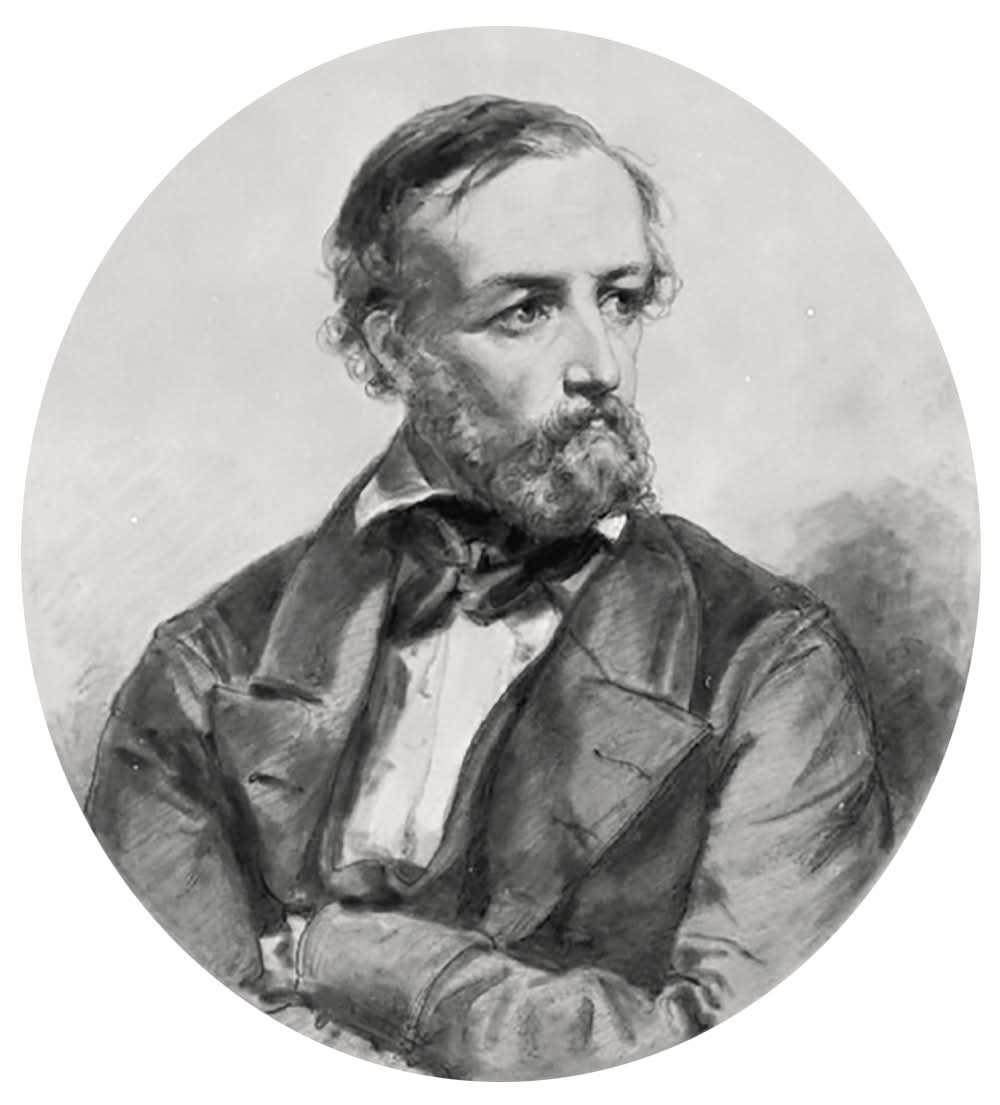
\includegraphics[scale=0.15]{img/pglDirichlet.jpg}
\caption{Peter Gustav Lejeune Dirichlet (1805-1859)}
\label{fig:pgl_dirichlet}
\end{figure}

\textbf{Definition:}
\begin{itemize}
    \item Pigeonhole sorting is a sorting algorithm that is suitable for sorting lists of elements where the number of elements and the number of possible key values are approximately the same.
    \item It requires $O(n + \text{Range})$ time where $n$ is the number of elements in the input array and ‘Range’ is the number of possible values in the array.
\end{itemize}

\subsection{Algorithm and Implementation}

Pigeonhole sort is similar to counting sort, but differs in that it “moves items twice: once to the bucket array and again to the final destination.

\begin{enumerate}
    \item \textbf{Determine the range:} Find minimum and maximum values in array. Let the minimum and maximum values be ‘min’ and ‘max’ respectively. Also find range as ‘max-min+1’.
    \item \textbf{Initialize an array:} Set up an array of initially empty “pigeonholes” the same size as of the range.
    \item \textbf{Distribution step:} Visit each element of the array and then put each element in its pigeonhole. An element $arr[i]$ is put in hole at index $arr[i] - \text{min}$.
    \item \textbf{Output reconstruction phase:} Start the loop all over the pigeonhole array in order and put the elements from non-empty holes back into the original array.
\end{enumerate}

\lstinputlisting[language=C++, caption=Pigeonhole Sort Algorithm, style=mystyle]{code/pigeonSort.cpp}

\subsection{Evaluation}

\subsubsection{Building the Pigeonhole Array}
\textbf{Operation:} Create and set up pigeonholes (buckets) for sorting the input array. \\
\textbf{Complexity:} \(O(n + \text{range})\) \\
\textbf{Explanation:} Each element in the input array is placed into its respective pigeonhole. The range refers to the difference between the maximum and minimum values.

\subsubsection{Filling the Pigeonhole Array}
\textbf{Operation:} Distribute elements from the input array into the pigeonholes. \\
\textbf{Complexity:} \(O(n)\) \\
\textbf{Explanation:} Traverse through the input array and assign each element to the appropriate pigeonhole.

\subsubsection{Reconstructing the Sorted Array}
\textbf{Operation:} Rebuild the sorted array by traversing through the pigeonholes in order. \\
\textbf{Complexity:} \(O(n + \text{range})\) \\
\textbf{Explanation:} Iterate over the pigeonholes and transfer elements back to the input array, ensuring the order is correct.

\subsubsection{Space Complexity Evaluation}
\textbf{Space Used:} \(O(\text{range})\) \\
\textbf{Explanation:} Additional memory is required to store the pigeonhole array, with its size being determined by the range of values in the input array (maximum value - minimum value + 1).

\subsection{Application}

Pigeonhole sort is a non-comparison-based sorting algorithm that works well for sorting integers or objects with small, discrete key ranges. It counts the occurrences of each element and uses this information to place elements in their correct sorted position.
\begin{enumerate}
    \item \textbf{Sorting Small Range Integers:} Pigeonhole sort is highly efficient for sorting integers or keys within a small, known range. \textit{Example:} Sorting exam scores (e.g., 0 to 100) or ages of individuals.
    \item \textbf{Histogram Generation:} Pigeonhole sort can be used to generate histograms or frequency distributions of data. \textit{Example:} Analyzing the frequency of words in a text or the distribution of pixel intensities in an image.
    \item \textbf{Data Compression:} Pigeonhole sort is used in data compression algorithms to analyze and organize data frequencies. \textit{Example:} Building frequency tables for Huffman coding or other compression techniques.
    \item \textbf{Counting Occurrences:} Pigeonhole sort can be used to count the occurrences of elements in a dataset. \textit{Example:} Counting the number of students who scored a particular grade in an exam.
    \item \textbf{Sorting Characters or Small Alphabets:} Pigeonhole sort is efficient for sorting characters or small alphabets. \textit{Example:} Sorting letters in a word or DNA sequences (A, T, C, G).
    \item \textbf{Real-Time Systems:} Pigeonhole sort is used in real-time systems where sorting needs to be done quickly and efficiently. \textit{Example:} Sorting sensor data in real-time for IoT devices.
    \item \textbf{Database Indexing:} Pigeonhole sort can be used in database systems to sort and index records with small key ranges. \textit{Example:} Sorting records by a small set of categories or flags.
    \item \textbf{Statistical Analysis:} Pigeonhole sort is used in statistical analysis to sort and analyze data distributions. \textit{Example:} Sorting survey responses or experimental data for further analysis.
    \item \textbf{String Sorting:} Pigeonhole sort is used in string sorting algorithms, especially when sorting by a specific character position. \textit{Example:} Sorting strings lexicographically or by a specific attribute.
\end{enumerate}

\subsection{Problems}

\subsubsection{Pigeonhole Sort 1}
\begin{itemize}
    \item \textbf{Description:} Sort an array of integers using pigeonhole sort.
    \item \textbf{Detailed Instructions:}
    \begin{enumerate}
        \item Identify the minimum and maximum values in the array to determine the range.
        \item Initialize a pigeonhole array of size \(\text{max} - \text{min} + 1\).
        \item Traverse the input array, placing each element in the corresponding pigeonhole.
        \item Reconstruct the sorted array by iterating through the pigeonhole array and placing elements back into the original array.
    \end{enumerate}
\end{itemize}

\subsubsection{The Full Pigeonhole Sort}
\begin{itemize}
    \item \textbf{Description:} Sort pairs of numbers and strings based on numeric keys while preserving the original order for equal keys.
    \item \textbf{Detailed Instructions:}
    \begin{enumerate}
        \item Create a pigeonhole array based on the numeric keys and place the elements in the corresponding pigeonholes.
        \item Reconstruct the sorted array by iterating through the pigeonhole array and placing elements back into the original array, ensuring stability.
    \end{enumerate}
\end{itemize}

\subsubsection{Find All Numbers Disappeared in an Array}
\begin{itemize}
    \item \textbf{Description:} Identify which numbers in the range [1, n] are missing from the input array.
    \item \textbf{Detailed Instructions:}
    \begin{enumerate}
        \item Create a boolean (or pigeonhole) array of size \(n+1\), initialized to mark all numbers as missing.
        \item Traverse the input array and mark each number that appears in the corresponding index of your boolean array.
        \item Iterate through the range 1 to \(n\) and collect those numbers that remain unmarked, as these are the missing numbers. This counting technique ensures that every potential number is checked exactly once.
    \end{enumerate}
\end{itemize}

\subsubsection{Sort an Array of 0s, 1s and 2s}
\begin{itemize}
    \item \href{https://www.geeksforgeeks.org/sort-an-array-of-0s-1s-and-2s/}{geeksforgeeks.org}
    \item \textbf{Description:} Sort an array containing only 0s, 1s, and 2s (a variant often used for the Dutch National Flag problem).
    \item \textbf{Detailed Instructions:}
    \begin{enumerate}
        \item Iterate over the array to count the number of 0s, 1s, and 2s.
        \item Overwrite the original array by placing the counted number of 0s first, followed by 1s and then 2s.
        \item Validate the resulting array to ensure that all elements are in the expected sorted order.
    \end{enumerate}
\end{itemize}

\subsubsection{Sort Characters By Frequency}
\begin{itemize}
    \item \href{https://leetcode.com/problems/sort-characters-by-frequency/}{LeetCode}
    \item \textbf{Description:} Rearrange the characters of a string so that characters with higher frequencies come first.
    \item \textbf{Detailed Instructions:}
    \begin{enumerate}
        \item Traverse the string to build a frequency map for each character.
        \item Use a bucket sort (pigeonhole sort style) where each bucket corresponds to a frequency, placing characters into the appropriate bucket.
        \item Reconstruct the string by iterating through the buckets from highest to lowest frequency, appending each character as many times as its frequency.
    \end{enumerate}
\end{itemize}

\subsubsection{Sort Array by Increasing Frequency}
\begin{itemize}
    \item \href{https://leetcode.com/problems/sort-array-by-increasing-frequency/}{LeetCode}
    \item \textbf{Description:} Sort the elements of an array by their frequency. In case of ties, the smaller number should come first.
    \item \textbf{Detailed Instructions:}
    \begin{enumerate}
        \item Count the frequency of each element using a hash map or count array.
        \item Create buckets where each bucket holds the elements corresponding to a specific frequency.
        \item Iterate through the buckets in ascending order of frequency; for tied frequencies, sort the numbers in ascending order, then rebuild the array from these sorted buckets.
    \end{enumerate}
\end{itemize}

\subsubsection{Sort Integers by The Number of 1 Bits}
\begin{itemize}
    \item \href{https://leetcode.com/problems/sort-integers-by-the-number-of-1-bits/}{LeetCode}
    \item \textbf{Description:} Sort integers by the number of 1s in their binary representation; if two numbers have the same number of 1s, sort them by their numeric value.
    \item \textbf{Detailed Instructions:}
    \begin{enumerate}
        \item For each integer, compute the number of 1 bits (this can be done using bit manipulation or a built-in function).
        \item Use these counts as keys for sorting. If two numbers have the same bit count, compare their numerical values.
        \item Reconstruct the sorted array based on these comparisons, ensuring that the algorithm is efficient by possibly caching bit counts for repeated values.
    \end{enumerate}
\end{itemize}
% \section{Thuật toán}
Dùng gói \texttt{algorithm} và \texttt{algpseudocode} để gõ đoạn thuật toán~\ref{alg:label}\footnote{Tất nhiên đây là dùng katana mổ ruồi!}

\begin{algorithm}
\caption{Thuật toán đếm xem nhiều gà hay nhiều chó hơn}
\label{alg:label}
\begin{algorithmic}
\Function {GaChoSoNaoLonHon}{\textit{ga}, \textit{cho}}
\State $soGa \gets 0$
\State $soCho \gets 0$
\For {$i \in [0, |ga| - 1]$}
\State $soGa \gets soGa + 1$
\EndFor
\For {$i \in [0, |cho| - 1]$}
\State $soCho \gets soCho + 1$
\EndFor

\If {$soGa > soCho$}
\State\Return $soGa$
\ElsIf {$soGa < soCho$}
\State\Return $soCho$
\Else 
\State\Return \texttt{"bang nhau"}
\EndIf
\EndFunction
\end{algorithmic}
\end{algorithm}
% \section{Code}
Dùng gói \texttt{listings} để gõ code, ví dụ cho C++:
\lstinputlisting[language=C++]{code/example.cpp}

Cho Python:
\lstinputlisting[language=Python]{code/example.py}

Đặc biệt: code có comment bằng tiếng Việt
\vietnameselst
\lstinputlisting[language=Python]{code/example-vietnamese.py}
% \section{Ngôn ngữ}
Ngôn ngữ mặc định của template là Tiếng Việt, config ở file \texttt{main.tex} với lệnh
\begin{lstlisting}[language=tex]
\usepackage[utf8]{vietnam}
\end{lstlisting}
Để chuyển sang Tiếng Anh (e.g. nhiều khi bạn muốn label trong các bảng bằng Tiếng Anh; bạn muốn viết report bằng Tiếng Anh thay vì Tiếng Việt), khi đó có 2 lựa chọn:
\begin{itemize}
\item Chuyển xang xài package \texttt{babel} và xài tag \texttt{$\backslash$uselanguage}.
\item Bỏ xài package \texttt{vietnam}
\end{itemize}
Hướng dẫn thì mời bạn xem \href{https://www.overleaf.com/learn/latex/International_language_support#Babel}{link này}
\section{Reference}

Example \cite{Thealgorithmsbundle}.

% References
\cleardoublepage
\phantomsection
\addcontentsline{toc}{section}{Tài liệu}
\bibliographystyle{plain}
\bibliography{ref/ref}

% Appendix
\appendix

\cleardoublepage
\section{Appendix}
\begin{itemize}
    \item Source code: \href{https://github.com/pnmq1103/cs163-seminar}{GitHub}
    \item Template source: \href{https://github.com/khongsomeo/hcmus-unofficial-report-template}{khongsomeo} 
    \item Reference: \href{https://github.com/tranlynhathao/fit-vnuhcmus_template}{tranlynhathao}
    \item Documentation: \href{https://mirror.unpad.ac.id/ctan/macros/latex/contrib/algorithms/algorithms.pdf}{The algorithms bundle}
\end{itemize}

\end{document}